\chapter{\textbf{Обзор литературы}}\label{ch:literature}
\section{\textbf{Одноэлектроное приближение}}
В качестве базового приближения выберем хорошо известное одноэлектронное приближение, являющееся составной частью
метода Хартри"--~Фока\cite{Hartree}. Его суть состоит в предположении о том, что волновая функция каждого электрона
может быть посчитана независимо.
В уравнение Шрёдингера вводится член, который учитывает взаимодействие электронов между
собой. Учет правильной симметрии волновой функции приводит к появлению в уравнениях
обменного потенциала, который обеспечивает соблюдение требования принципа Паули
(уравнения с обменным потенциалом "---и есть уравнения Хартри-Фока).
Кроме того, кулоновское поле считается центрально"=симметричным, что позволяет провести
соответствующее разделение переменных при решении уравнения Шрёдингера.

Таким образом, волновую функцию многоэлектронной системы, по теореме произведения вероятностей, можно представить как
произведение волновых функций отдельных электронов:
\begin{equation}\label{eq:hartree}
  \Psi(\mathbf{r_1}, \mathbf{r_2}, \dots, \mathbf{r_N}) =
  \psi_1(\mathbf{r_1}) \psi_2(\mathbf{r_2}) \dots \psi_3(\mathbf{r_3}),
\end{equation}

где N "---число электронов в системе.

Эта идея использовалась первоначально Д. Хартри.
У такого представления, однако, есть существенный недостаток: перестановка любых
двух радиус"=векторов электронов в данной формуле не изменит знака результирующей
волновой функции, что противоречит принципу Паули. Для того, чтобы это исправить,
формулу \eqref{eq:hartree} можно переписать в следующем виде\cite{Davidov}:
\begin{equation}\label{eq:fockWaveFunction}
  \Psi(\mathbf{r_1}, \mathbf{r_2}, \dots, \mathbf{r_N}) =
  \frac{1}{\sqrt{N!}}
  \begin{vmatrix}
    \psi_1(\mathbf{r_1}) & \psi_2(\mathbf{r_1}) & \cdots & \psi_N(\mathbf{r_1})\\
    \psi_1(\mathbf{r_2}) & \psi_2(\mathbf{r_2}) & \cdots & \psi_N(\mathbf{r_2})\\
    \vdots & \vdots & \ddots & \vdots\\
    \psi_1(\mathbf{r_N}) & \psi_2(\mathbf{r_N}) & \cdots & \psi_N(\mathbf{r_N})
  \end{vmatrix}.
\end{equation}

Теперь при любой замене вида
\begin{equation}
  \begin{split}
    \mathbf{r_i} \rightarrow \mathbf{r_j}\\
    \mathbf{r_j} \rightarrow \mathbf{r_i}
  \end{split}
\end{equation}

строки в определителе поменяются местами, и волновая функция
$\Psi(\mathbf{r_1}, \mathbf{r_2}, \dots, \mathbf{r_N})$ сменит знак.

Выделяют ограниченный и неограниченный методы Хартри"--~Фока. В первом полагается, что
каждая орбиталь занята парой электронов с различными спинами. Такой метод проще в
реализации, однако, вышеописанное допущение не соблюдается при рассмотрении систем с
незаполненными оболочками, так как в них обменные потенциалы для разных проекций спина различны.
При этом плотности электронов с разными проекциями спинов смещаются относительно друг друга и возникает разность
плотностей "---спиновая плотность $\rho^{\sigma}(\mathbf{r})$. Для описания магнитных эффектов необходимо учитывать это
обстоятельство\cite{Pople}.

\section{\textbf{Локальный обменный потенциал Слейтера}}
Одним из членов гамильтониана многоэлектронной системы является
обменный потенциал. Эта величина обладает свойством нелокальности
"---она зависит от волновой функции системы электронов, поэтому уравнение
для нахождения волновой функции становится интегро"=дифференциальным, что сильно усложняет
расчёты.

Проблему можно решить, если приблизить нелокальный обменный потенциал локальным аналогом.
Слейтер, пользуясь моделью однородного электронного газа, предложил две формулы для локального потенциала:
не учитывающую эффект спиновой поляризации
\begin{equation}\label{eq:SlaterExchange}
  \widehat{V}_X(\mathbf{r}) = 3 \left(
    \frac{ 3 }{ 8 \pi }
    \rho(\mathbf{r})
  \right)^{1/3}
\end{equation}

и учитывающую
\begin{equation}
  \widehat{V}_X^{\sigma}(\mathbf{r}) = 3 \left(
    \frac{ 3 }{ 4 \pi }
    \rho^{\sigma}(\mathbf{r})
  \right)^{1/3}.
\end{equation}

В обоих случаях $\rho(\mathbf{r})$ "---плотность электронов в точке с радиус"=вектором $\mathbf{r}$.

\section{\textbf{Обменный потенциал Гашпара"--~Кона"--~Шэма}}
Согласно теоремам Хоэнберга"--~Кона полную энергию системы электронов, находящихся во внешнем
потенциале $V(\mathbf{r})$, можно представить в виде функционала электронной плотности\cite{Hohenberg}:
\begin{equation}
  E[\rho] = \int{ V(\mathbf{r}) \rho(\mathbf{r}) d\mathbf{r} } + F[\rho],
\end{equation}

Пользуясь этим представлением можно вывести\cite{Gaspar}\cite{Kohn} выражение для локального обменного потенциала вида
\begin{equation}\label{eq:GashparKohnShamExchange}
  \widehat{V}_X(\mathbf{r}) = 2 \left(
    \frac{ 3 }{ 8 \pi }
    \rho(\mathbf{r})
  \right)^{1/3}.
\end{equation}

Формула \eqref{eq:GashparKohnShamExchange} совпадает с \eqref{eq:SlaterExchange}
с точностью до постоянного множителя "---обменный потенциал Гашпара"--~Кона"--~Шэма
оказался в полтора раза слабее обменного потенциала Слейтера; как следствие, электроны располагаются
дальше от ядер. Было показано, что такой выбор обменного потенциала приводит к
лучшему согласию с экспериментом, чем обменный потенциал Слейтера, в частности, он более пригоден для описания
химических связей\cite{nyavro}.

\section{\textbf{Обменный потенциал Гуннарссона"--~Лундквиста}}
В данной работе наибольший интерес представляет использование обменного потенциала Гуннарссона"--~Лундквиста\cite{GUNNARSSON1976177},
поскольку
он хорошо зарекомендовал себя при изучении магнитных свойств молекул и кластеров\cite{nyavro}. При его выводе используются
всё те же теоремы Хоэнберга"--~Кона, но в гамильтониан также вводится член, зависящий от температуры. В его формулы
явно входят спиновые плотности электронов, что позволяет корректно учитывать эффект спиновой поляризации, обуславливающий появление магнетизма.

Практически расчёт потенциала Гуннарссона"--~Лундквиста состоит в следующем. Прежде всего вводится понятие относительной спиновой поляризации
\begin{equation}
  \zeta(\mathbf{r}) = \frac{\rho^\uparrow({\mathbf{r}}) - \rho^\downarrow({\mathbf{r}})}{\rho({\mathbf{r}})},
\end{equation}
где $\rho^\uparrow({\mathbf{r}})$ "---плотность электронов со спином "вверх" и $\rho^\downarrow({\mathbf{r}})$
"---плотность электронов со спином "вниз".

Затем рассчитываются вспомогательные перменные:
\begin{equation}
  \gamma = 0.297,
\end{equation}

\begin{equation}
  \beta = 1 + 0.0545 r_s ln\left( 1 + \frac{11.4}{r_s} \right),
\end{equation}

\begin{equation}
  \delta = 1 - 0.036 r_s + \frac{1.36 r_s}{1 + 10 r_s},
\end{equation}

\begin{equation}
  r_s = \left( \frac{3}{4\pi} \frac{1}{\rho(\mathbf{r})} \right).
\end{equation}

И наконец, сам потенциал Гуннарссона"--~Лундквиста может быть расчитан по формуле
\begin{equation}
  V^{\sigma}_{XGL} = V_{XGKS}(\mathbf{r}) \left( \beta \pm \frac{1}{3} \frac{\delta \zeta}{1 \pm \gamma \zeta} \right).
\end{equation}

\section{\textbf{Метод присоединённых плоских волн}}
При разложении волновых функций электронов в кристаллах разумно использовать
в качестве базисных функции, точно удовлетворяющие теореме Блоха "---плоские
волны. Однако, такое разложение плохо сходится вблизи атомов, так как потенциал
здесь очень сильно меняется, как следствие, нужно использовать очень
большое число плоских волн для того, чтобы достичь требуемой точности
вычислений. С другой стороны, в области между атомами потенциал меняется слабо,
он практически постоянен, и разложение по плоским волнам оказывается вполне
адекватной процедурой. Схематическая демонстрация вышесказанного изображена
на рисунке~\ref{fig:muffintin} (ямы в центре каждой ячейки на самом деле уходят
в минус бесконечность, но на рисунке они обрезаны).
\begin{figure}[ht]
  \centerfloat{
    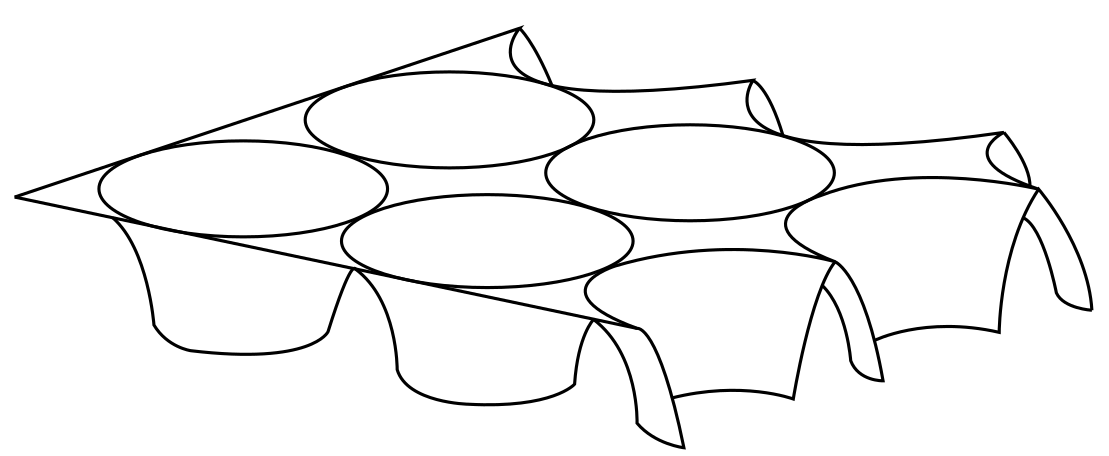
\includegraphics[scale=1.0]{muffintin}
  }
  \caption{Схематическое изображение MT"=потенциала, векторизация рисунка из \cite{Harrison}}
  \label{fig:muffintin}
\end{figure}

Поэтому\cite{afw-method}\cite{SlaterSimplification} Слейтер предложил кристаллический потенциал $V(r)$ представлять в виде
\begin{equation}
  V(r) =
  \begin{cases}
    V'(r), & r \le R_{Mt}^s \\
    V_c, & r > R_{Mt}^s
  \end{cases}
\end{equation}

Для простоты положим $V_c = 0$. В нулевом приближении кристаллическую плотность
электронов можно представить в виде суммы атомных плотностей:
\begin{equation}\label{eq:afw-method-1}
  \rho^{\text{кр}}(\mathbf{r}) = \sum_A {
    \rho^{\text{ат}} \left(\mathbf{r} - \mathbf{R^s}\right)
  }
\end{equation}

Волновая функция электрона с радиус"=вектором $\mathbf{r}$ параметризована
вектором $\mathbf{k_i}$ и внутри MT"=сферы записывается как
\begin{equation}\label{eq:afw-method-2}
  \phi^1(\mathbf{k_i}, \mathbf{r}) = \sum_{l = 0}^{\infty} {
    \sum_{m = -l}^{l} {
      A_{lm}(\mathbf{k_i}) R_l(E, r) Y_{lm}(\mathbf{\widehat{k}_i})
    }
  },
\end{equation}

где $R_l(E, r)$ "--- решение радиального уравнения
\begin{equation}\label{eq:radialEquation}
  \left[{
    -\frac{1}{r^2} \frac{d}{dr} \left({
      r^2 \frac{d}{dr}
    }\right) + \frac{l\left(l + 1\right)}{r^2} + V(r) - E
  }\right] R_l(E, r) = 0, r \le R_{Mt}^s,\
\end{equation}

$A_{lm}(\mathbf{k_i})$ "---коэффициенты разложения, точный вид которых будет
определён чуть позже.

Волновая функция электрона вне MT"=сферы записывается как
\begin{equation}\label{eq:afw-method-3}
  \phi^{2}(\mathbf{k_i}, \mathbf{r}) = e^{
    i\mathbf{k_i} \left( \mathbf{R^s} + \mathbf{r} \right)
  }, r > R_{mt}^s.
\end{equation}

Плоскую волну представим в виде разложения по сферическим функциям Бесселя
\begin{equation}\label{eq:afw-method-4}
  e^{ i\mathbf{k_i} \left( \mathbf{R^s} + \mathbf{r} \right) } =
  4 \pi e^{i \mathbf{k_i} \mathbf{R^s}}
  \sum_{l = 0}^{\infty} {
    \sum_{m = -l}^{l} {
    i^l j_l(k_i r) Y_{lm}^{*}(\mathbf{\widehat{k}_i}) Y_{lm}(\mathbf{\widehat{r}})
    }
  }.
\end{equation}

Из условия сшивания волновой функции на границе MT"=сферы получается выражение
для коэффициентов
\begin{equation}
  A_{lm}(\mathbf{k_i}) = 4 \pi e^{i \mathbf{k_i} \mathbf{R^s}}
  i^l j_l(k_i R_{mt}^s) Y_{lm}^{*}(\mathbf{\widehat{k}_i})
  \frac{1}{R_l(E, R_{mt}^s)}.
\end{equation}

Спектр волновой функции находится из условия минимума определителя матрицы
$M_{ij}$, составленной по следующему принципу:
\begin{equation}\label{eq:afw-method-5}
  M_{ij} = (\mathbf{k_i}\mathbf{k_j} - E)\delta_{ij} -
  \sum_s{
    \frac{3 \pi (R_{mt}^s)^2}{R_0^3}
    e^{\left\lvert \mathbf{k_i} - \mathbf{k_j} \right\lvert R^s}
    F_{ij,s}
  },
\end{equation}

где $R_0$ "---радиус атома,
\begin{equation}\label{eq:afw-method-6}
  F_{ij,s} =
    (\mathbf{k_i}\mathbf{k_j} - E)
    \frac
      {j_1(\left\lvert \mathbf{k_i} - \mathbf{k_j} \right\lvert R_{mt}^s)}
      {\left\lvert \mathbf{k_i} - \mathbf{k_j} \right\lvert}
    - \sum_{l = 0}^{\infty} {
      P_l(\widehat{\mathbf{k_i}, \mathbf{k_j}})
      j_l(k_i R_{mt}^s)
      j_l(k_j R_{mt}^s)
      \frac{ R_l'(E, R_{mt}^s) }{ R_l(E, R_{mt}^s) }
    }.
\end{equation}

\section{\textbf{Метод рассеянных волн}}
Метод рассеянных волн\cite{sw-method} во многом схож с методом присоединённых плоских волн. Точно так же пространство
делится на атомные и межатомные области, волновые функции в которых находятся независимо друг от друга, а затем
сшиваются, различие же состоит в выборе базисных функций для межатомных областей.

Полная формулировка метода рассеянных волн включает в себя, помимо упомянутых двух областей, также внешнюю область,
лежащую за так называемой сферой Неймана. Однако, учёт этой сферы только портит результаты в случае больших атомных
систем или же атомных систем с большой ассиметрией. Именно такие системы изучаются в данной работе, поэтому опустим
рассмотрение этой сферы.

В отличие от метода присоединённых плоских волн в данном методе используется большее число спец.функций, а именно:
\begin{enumerate}
  \item Обыкновенные сферические функции Бесселя $j_l(x)$.
  \item Обыкновенные сферические функции Неймана (также называемые обыкновенными сферическими функциями Бесселя второго
  рода) $n_l(x)$.
  \item Модифицированные сферические функции Бесселя первого рода $i_l(x)$.
  \item Модифицированные сферически функции Ганкеля первого рода $k_l^{(1)}(x)$.
\end{enumerate}

В атомных областях волновые функции, аналогично методу присоединённых плоских волн, раскладываются по атомным функциям:
\begin{equation}
  \psi_1^p(\mathbf{r}) = \sum_L{C_L^p R_l^p(E, r) Y_L(\mathbf{r})},
\end{equation}
где $L$ "---упорядоченная пара коэффициентов $(l, m)$, которые меняются по правилу $l \in [0, 2]$, $m \in [0, l]$;
$Y$ "---вещественная сферическая функция, $C_L^p$ "---коэффициенты, которые будут определены в дальнейшем, $p$ "---индекс
атома.

В межатомных областях волновые функции раскладываются следующим образом:
\begin{equation}
  \psi_2(\mathbf{r}) = \sum_j{\sum_L{A_L^p k_l^{(1)}(\kappa r_p) Y_L(\mathbf{r})}},
\end{equation}

где
\begin{equation}
  \kappa = \sqrt{|E - \overline{V}_{II}|},
\end{equation}

\begin{equation}
  \overline{V}_{II} = \frac{1}{\Omega_{II}} \int_{\Omega_{II}}{V(\mathbf{r}) d\mathbf{r}},
\end{equation}

$\Omega_{II}$ "---межатомный объём.

Для нахождения спектра составляется матрица как функция энергии. Матрица является двумерной, а её индексы "---это
упорядоченные тройки $(p, l, m)$.

Диагональные элементы находятся по следующему принципу:
\begin{equation}
  t_l^p(E) = - \frac{
    W[ i_l(\kappa b_j), R_l^p(E, b_j)]
  }{
    W[ k_l^{(1)}(\kappa b_j), R_l^p(E, b_j)]
  }, E < \overline{V}_{II},
\end{equation}
\begin{equation}
  t_l^p(E) = - \frac{
    W[ j_l(\kappa b_j), R_l^p(E, b_j)]
  }{
    W[ n_l(\kappa b_j), R_l^p(E, b_j)]
  }, E > \overline{V}_{II},
\end{equation}

где
\begin{equation}
  W[ u(x), v(x) ] = u\frac{dv(x)}{dx} - \frac{du(x)}{dx}v,
\end{equation}

а $b_j$ "---радиус атомной сферы атома с индексом p.

Недиагональные элементы матрицы находятся по формулам (здесь символы без штриха и со штрихом "---элементы горизонтальных
и вертикальных индексов матрицы)
\begin{equation}
  G_{LL'}^{pp'}(E) = (1 - \delta_{pp'}) 4 \pi (-1)^{l + l'} \sum_{L''}{I_{L''}(L; L')} k_{l''}^{(1)}(\kappa |\mathbf{R_{pp'}}|)
  Y_{L''}(\mathbf{R_{pp'}}), E < \overline{V}_{II},
\end{equation}

\begin{equation}
  G_{LL'}^{pp'}(E) = (1 - \delta_{pp'}) 4 \pi i^{l - l'} \sum_{L''}{i^{-l''} I_{L''}(L; L')} n_{l''}(\kappa |\mathbf{R_{pp'}}|)
  Y_{L''}(\mathbf{R_{pp'}}), E < \overline{V}_{II},
\end{equation}

где $\mathbf{R_{pp'}}$ "---векторы, соединяющие центры атомов с соответствующими индексами, а $I_{L''}(L; L')$ "---интегралы
Гаунта:
\begin{equation}\label{eq:gaunt}
  I_{L''}(L; L') = \int_0^{2\pi} {d\phi \int_0^{\pi}{
  Y_{L''}(\theta, \phi) Y_{L}(\theta, \phi) Y_{L'}(\theta, \phi)
  \, \sin \theta d\theta
  }}.
\end{equation}

Спектр заданной атомной системы находится из условия равенства детерминанта построенной таким образом матрицы нулю.
Далее, из решения секулярного уравнения, построенного с помощью этой матрицы, а также из условия сшивания волновых
функций на границе атомных и межатомных областей находятся коэффициенты $A_L^p$ и $C_L^p$.

\FloatBarrier
